% Part: sets-functions-relations
% Chapter: relations
% Section: graphs

\documentclass[../../../include/open-logic-section]{subfiles}

\begin{document}

\olfileid{sfr}{rel}{grp}
\olsection{Grafen}

Een \emph{graaf} is een tekening waarin punten met lijnen aan elkaar
zitten. De punten heten ‘knopen’ of ‘knooppunten’; ‘knooppunten’ is het
meervoud van ‘knooppunt’. Grafen kom je overal tegen in de discrete
wiskunde en de informatica. Ze laten zien welke dingen met elkaar
verbonden zijn en hoe iets in elkaar zit. Dat kan iets tastbaars zijn,
zoals allerlei netwerken, maar ook iets dat alleen in gedachten bestaat,
zoals alles wat een beslissing kan opleveren. Er bestaan veel soorten
grafen.
Soms hebben de lijnen een richting of een label, soms niet. Soms mag
een lijn bij hetzelfde punt uitkomen waar hij begon, en soms mogen
tussen dezelfde punten meer lijnen lopen. \emph{Gerichte grafen},
waarin de lijnen een richting hebben, hangen op een bijzondere manier
samen met relaties.

\begin{defn}[Gerichte graaf]
Een \emph{gerichte graaf} $G = \tuple{V, E}$ heeft een verzameling
\emph{knopen}~$V$ en een verzameling \emph{pijlen}~$E \subseteq V^2$.
\end{defn}

\begin{explain}
Volgens de definitie is een graaf gewoon een verzameling met een
relatie op die verzameling. Bij een graaf verwachten we natuurlijk
een tekening. We tekenen precies dan een pijl van knoop~$v_1$ naar
knoop~$v_2$ als $\tuple{v_1, v_2} \in E$. Een losse relatie zegt niet
apart welke knopen erbij horen; een graaf doet dat wel. Daarom kan een
graaf ook knopen hebben waar geen pijl aankomt of vertrekt. Het
belangrijkste is dat we elke relatie~$R$ op een verzameling~$X$ kunnen
zien als de gerichte graaf $\tuple{X, R}$. Andersom kunnen we een
gerichte graaf~$\tuple{V, E}$ zien als een relatie $E \subseteq V^2$,
waarbij de verzameling $V$ er apart bij staat.
\end{explain}

\begin{ex}
Zo ziet de graaf $\tuple{V, E}$ met $V = \{1, 2, 3, 4\}$ en $E =
\{\tuple{1,1}, \allowbreak \tuple{1, 2}, \allowbreak \tuple{1, 3},
\allowbreak \tuple{2, 3}\}$ eruit:
\begin{align*}
& 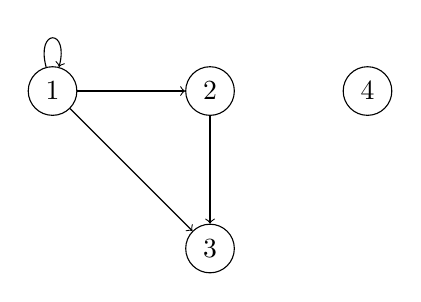
\begin{tikzpicture}[->,node distance=2cm]
  \node[draw,circle] (A) {$1$};
  \node[draw,circle] (B) [right of=A] {$2$};
  \node[draw,circle] (C) [below of=B] {$3$};
  \node[draw,circle] (D) [right of=B] {$4$};
  \draw (A) to [loop above]  (A);
  \draw (A) to  (B);
  \draw (A) to  (C);
  \draw (B) to  (C);
  \end{tikzpicture}
\intertext{Dit is niet dezelfde graaf als $\tuple{V', E}$ met $V' =
  \{1, 2, 3\}$. Die ziet er zo uit:}
& 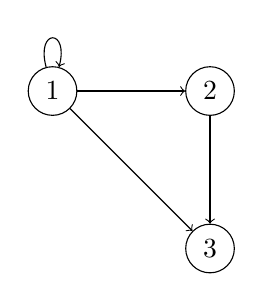
\begin{tikzpicture}[->,node distance=2cm]
  \node[draw,circle] (A) {$1$};
  \node[draw,circle] (B) [right of=A] {$2$};
  \node[draw,circle] (C) [below of=B] {$3$};
  \draw (A) to [loop above]  (A);
  \draw (A) to  (B);
  \draw (A) to  (C);
  \draw (B) to  (C);
  \end{tikzpicture}
\end{align*}
\end{ex}

\begin{prob}
  Zie de relatie ‘kleiner dan of gelijk aan’~$\le$ op de verzameling
  $\{1, 2, 3, 4\}$ als een graaf. Teken hoe die graaf eruitziet.
\end{prob}
\end{document}
